\renewcommand{\theequation}{\theenumi}
\begin{enumerate}[label=\arabic*.,ref=\thesubsection.\theenumi]
\numberwithin{equation}{enumi}
\item Finding the equation of angular bisectors if $\vec{A}, \vec{B}, \vec{C}$ are given, where
$\vec{BD}$ is the angular bisector.
\\
\solution To find the equation of the bisector $\vec{BD}$.
\\ 
From the figure \ref{fig:proof}, let $\vec{B}$ be origin, and 
\begin{align}
\vec{P_1}=\frac{\vec{C}}{\norm{\vec{C}}}
\\
\vec{P_2}=\frac{\vec{A}}{\norm{\vec{A}}}
\end{align}
\begin{figure}[!ht]
	\begin{center}
			\resizebox{\columnwidth}{!}{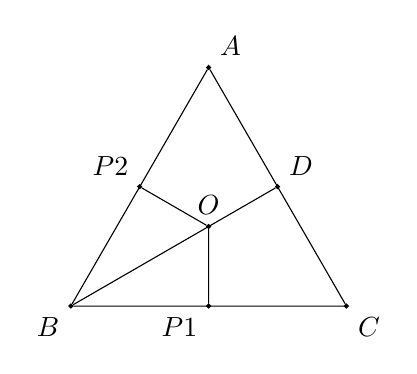
\begin{tikzpicture}
[scale=1.75,>=stealth,point/.style={draw,circle,fill = black,inner sep=0.5pt},]

%Triangle sides




%Labeling points
\node (A) at (1,1.732)[point,label=above right:$\tiny A$] {};
\node (B) at (0, 0)[point,label=below left:$\tiny B$] {};
\node (C) at (2, 0)[point,label=below right:$\tiny C$] {};
\node (O) at (1,0.577)[point,label=above:$\tiny O$] {};
\node (D) at (1.5,0.866)[point,label=above right:$\tiny D$] {};
\node (P1) at (1,0)[point,label=below left:$\tiny P1$] {};
\node (P2) at (0.5,0.866)[point,label=above left:$\tiny P2$] {};

%Drawing triangle ABC
\draw (A) -- node[left] {$\textrm{}$} (B) -- node[below] {$\textrm{}$} (C) -- node[above,xshift=5mm] {$\textrm{}$} (A);


%Joining BD
\draw (B)--(D);
\draw (O)--(P1);
\draw (O)--(P2);

%Drawing and marking angles
%\tkzMarkAngle[fill=orange!10,mark=||](D,B,A)
%\tkzMarkAngle[fill=orange!10,mark=||](C,B,D)
%\tkzMarkAngle[fill=green!40,size=0.5cm,mark=](A,B,C)
\tkzMarkRightAngle[fill=blue!20](O,P1,B)
\tkzMarkRightAngle[fill=blue!20](O,P2,B)
%\tkzLabelAngle[pos=0.25](D,B,A){$\theta$}
%\tkzLabelAngle[pos=0.25](C,B,D){$\theta$}
%\tkzLabelAngle[pos=0.65](A,B,C){$\alpha$}


\end{tikzpicture}

}
	\end{center}
	\caption{Triangle with angular bisectors.}
	\label{fig:proof}	
\end{figure}
Then $\vec{P_1}\vec{P_2} \perp \vec{BD}$
\begin{align}
\label{eq:1}
\vec{D}^T \brak{\vec{P_1}-\vec{P_2}} = 0
\end{align}
However, $\norm{\vec{P_1}}=\norm{\vec{P_2}}$
\\
$\implies \brak{\norm{\vec{P_1}}}^2=\brak{\norm{\vec{P_2}}}^2$
\\
$\implies \brak{\vec{P_1}-\vec{P_2}}^T \brak{\vec{P_1}+\vec{P_2}}=0$
\begin{align}
\label{eq:2}
\implies \vec{P_1}+\vec{P_2} \perp \vec{P_1}-\vec{P_2}
\end{align}
From \ref{eq:1} and \ref{eq:2} 
\begin{align}
\vec{D}=k \brak{\vec{P_1}+\vec{P_2}}
\end{align}
Then equation of $\vec{BD}$ is:
\begin{align}
\vec{BD}: \vec{x}=\lambda \brak{\vec{P_1}+\vec{P_2}} 
\\
\label{const:proof}
\vec{x}= \lambda \brak{\frac{\vec{A}}{\norm{\vec{A}}}+\frac{\vec{C}}{\norm{\vec{C}}}}
\end{align}
If $\vec{B}$ is not at origin then,
\begin{align}
\vec{BD}: \vec{x}=\vec{B}+\lambda \brak{\frac{\vec{A}-\vec{B}}{\norm{\vec{A}-\vec{B}}}+\frac{\vec{C}-\vec{B}}{\norm{\vec{C}-\vec{B}}}}
\end{align}

\end{enumerate}
